\documentclass[12pt, letterpaper]{article}
\usepackage[margin=0.5in]{geometry}

\usepackage{graphicx}
\usepackage[utf8]{inputenc}
\usepackage{listingsutf8}
\usepackage[T1]{fontenc}
\usepackage{xcolor}
\usepackage{hyperref}
\usepackage{float}

% For math purpuse
\usepackage{amsmath}
\usepackage{amssymb}
\usepackage{pgfplots}

\usepackage{listings}
\lstset{
    language=Python,
    basicstyle=\ttfamily\small,
    aboveskip={1.0\baselineskip},
    belowskip={1.0\baselineskip},
    columns=fixed,
    extendedchars=true,
    breaklines=true,
    tabsize=4,
    prebreak=\raisebox{0ex}[0ex][0ex]{\ensuremath{\hookleftarrow}},
    frame=lines,
    showtabs=false,
    showspaces=false,
    showstringspaces=false,
    keywordstyle=\color[rgb]{0.627,0.126,0.941},
    commentstyle=\color[rgb]{0.133,0.545,0.133},
    stringstyle=\color[rgb]{01,0,0},
    numbers=left,
    numberstyle=\small,
    stepnumber=1,
    numbersep=10pt,
    captionpos=t,
    escapeinside={\%*}{*n)
    }}
  
\graphicspath{{img/}}

\title{CENTRO UNIVERSITARIO DE CIENCIAS EXACTAS E INGENIERIAS\\
  SEMINARIO DE ALGORITMIA\\
  \textbf{Actividad 11 Regresión Lineal:}}
\author{Sección: D11\\
  Alumno: Erick Alejandro Carrillo López\\
  Código: 221349828}

\date{2023/04/24}

\begin{document}
\maketitle
\tableofcontents
\newpage
\section{Introducción:}
\subsection{¿Que es una regresión lineal?:}
Realizar la regresión lineal es paso importante para introducirte en la inteligencia artificial, para
mí es como hacer un hello world en un lenguaje de programación, sus conceptos he ideas en los que se fundamenta
el algoritmo pueden ser algo 
complicadas para la gente que no esta familiarizada con las matemáticas.\\\\
En estadística, la regresión lineal es un enfoque lineal para modelizar la
relación entre una respuesta escalar y una o más variables explicativas, en palabras mas simples
busca una relación entre la variable dependiente con la independiente.\\\\
En el caso de que solo sea una variable independiente se dice que es una \textbf{regresión lineal simple}
pero para multiples variables independientes se dice que es una \textbf{regresión lineal multiple},
como tal es a travez de esta realación escalar que se busca modelar una \textbf{funcion lienal predictora},
que como su nombre lo dice busca predecir o aproximar sus \textbf{outcomes} a todas las
posibles variables dependientes.

\begin{figure}[H]
  \centering
  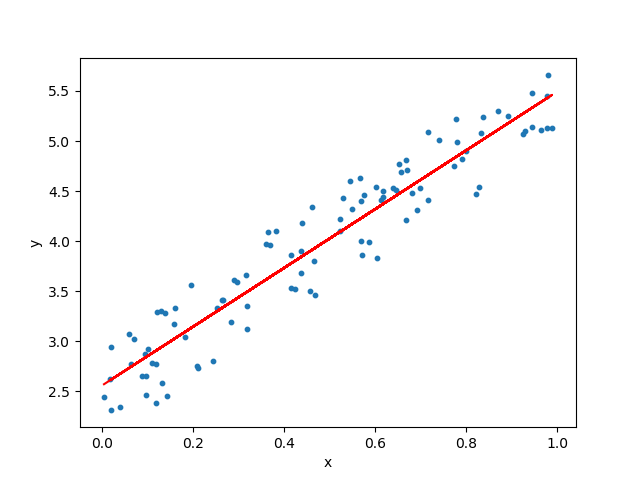
\includegraphics[scale = 0.5]{regression.png}
\end{figure}

Esta imagen representa perfectamente lo que se quiere logar a travez de la regresión lineal,
la linea roja representa la \textbf{funcion lineal predictora} que mejor se acomoda o ajusta a los datos
, esto a travez de una relación escalar.
\subsection{¿Cómo funciona?:}
El cómo funciona parte de la conjetura o hipótesis de que exista una función lineal dada en $\vec{x}$
que se ajuste mejor a los datos
o puntos por medio de una relación \textbf{escalar}, cuando digo relación escalar
me refiero a una
regla la cual puedes pensar en una función que pase de vectores a escalares.
\[
  E: \mathbb{R}^j \rightarrow \mathbb{R}
\]
Para ser exactos estoy hablando del \textbf{error cuadrático medio}, por la cual
fácilmente podemos proponer posibles  \textbf{funciones lineales predictoras} y medir su grado
de a proximidad al ajuste perfecto.
\[
  MES = \frac{1}{n} \cdot \sum^{n}_{i = 0} (y_i - \theta(\vec{x_i}))^2
\]
Donde $\theta(\vec{x_i}) = \vec{m} \cdot \vec{x_i}$ esta es la función lineal como puedes ver
simplemente es un producto punto, esta
recibe un vector con esta forma $\vec{x_i} = [1, x_1, \cdots, x_j]\quad |\quad x_0 = 1$
y este se multiplica por otro vector $\vec{m} = [b, m_1, \cdots, m_j]\quad |\quad m_0 = b$ por lo que
sustituimos podemos definir nuestra función como.
\[
  E(\vec{m}) = \frac{1}{n} \cdot \sum^{n}_{i = 0} ((\vec{m} \cdot \vec{x_i}) - y_i)^2
\]
Lógicamente, se eleva al cuadrado para evitar generar esas diferencias negativas y se pueda manejar 
esta como cantidad medible entonces si creamos un gráfico de esta función debería de verse como una
parábola, dentro del algoritmo de regresión lineal a esta función  se le conoce como función de coste.\\

\begin{center}
\begin{tikzpicture}
\begin{axis}[
  xlabel=$\vec{m}$,
  ylabel=$E(\vec{m})$,
  xmin=-5,xmax=5,
  ymin=-1,ymax=10,
  axis lines=center,
  domain=-3:3,
  samples=100,
  xtick=\empty, % removes numbers from x-axis
  ytick=\empty, % removes numbers from y-axis
]
\addplot+[mark=none] {x^2+2};
\end{axis}
\end{tikzpicture}
\end{center}

\subsection{El decenso del gradiente:}
El algoritmo funciona partiendo de un $\vec{m_0}$ con la forma $[b, m_1, \cdots, m_j]$
este se escoge de forma aleatoria
dentro del rango de la función $E(\vec{m})$, despues vamos a calcular la derivada 
de $E(\vec{m})$ sobre
$\vec{m}$, esta derivada en realidad es un \textbf{gradiente} un simple vector con multiples
derivadas parciales.
\[
  \frac{dE}{d\vec{m}} = \begin{bmatrix} \frac{\partial E}{\partial m_0} \\ \frac{\partial E}{\partial m_1}
                         \\ \vdots \\ \frac{\partial E}{\partial m_j} \end{bmatrix} = \nabla E
\]
Usando el \textbf{gradiente} podemos encontrar ese vector deseado el cual es $\vec{m}^*$,
este debería de ubicarse en el punto donde todas las derivadas parciales da las componentes dan cero.
\[
  \nabla E(\vec{m}^*) = \begin{bmatrix} \frac{\partial E}{\partial m^*_0}
                              \\ \frac{\partial E}{\partial m^*_1}
                              \\ \vdots
                              \\ \frac{\partial E}{\partial m^*_j} \end{bmatrix} =
                            \begin{bmatrix} 0
                              \\ 0
                              \\ \vdots
                              \\ 0 \end{bmatrix}
\]
                        
Y esto se debe a la ubicación del vector ideal $\vec{m}^*$ se encuentra en el punto más bajo de la parábola
de múltiples dimensiones.
\begin{center}
\begin{tikzpicture}
\begin{axis}[
  xlabel=$\vec{m}$,
  ylabel=$E(\vec{m})$,
  xmin=-5,xmax=5,
  ymin=-1,ymax=10,
  axis lines=center,
  domain=-3:3,
  samples=100,
  xtick=\empty, % removes numbers from x-axis
  ytick=\empty, % removes numbers from y-axis
]
\addplot+[mark=none] {x^2+2};
\node[label={below left:$\vec{m}^*$}, circle,fill,inner sep=2pt] at (axis cs:0,0) {};
\draw[thick] (250, 30) -- (750, 30);
\node[label={below left:$\scriptstyle \nabla E(\vec{m}^*) = [0, \cdots, 0]$}] at (axis cs:0,2) {};
\end{axis}
\end{tikzpicture}
\end{center}
\subsection{Calculando las derivadas parciales del gradiente:}
Ahora para calcular el gradiente debemos de calcular todas las derivadas parciales a través de las cuales
podemos usar la regla de la cadena para simplificar todos nuestros caculos.\\\\
Primero quiero desglosar un poco nuestra función de coste para entender mejor las derivadas parciales.
\[
  E(\vec{m}) = \frac{1}{n} \cdot \sum_{i = 0}^{n}(\vec{x_i} \cdot \vec{m} - y_i)^2 =
  \frac{1}{n} \cdot ((\vec{x_0} \cdot \vec{m} - y_0)^2 + \cdots + ( \vec{x_n} \cdot \vec{m} - y_n)^2)
\]
Recordemos que por cada $\vec{x_i} \cdot \vec{m}$ es un producto punto por lo que.
\[
  \vec{x_i} \cdot \vec{m}  = \sum_{l = 0}^{j} (x_{i, l} \cdot m_l)
\]
Sustituyendo nos debería de verse algo como esto.
\[
  E(\vec{m})
  = \frac{1}{n} \cdot ((\sum_{l = 0}^{j} (x_{0, l} \cdot m_l) - y_0)^2 +
  \cdots + (\sum_{l = 0}^{j} (x_{n, l} \cdot m_l) - y_n)^2)
\]
Por lo que si queremos calcular la derivada parcial para cualquier componente $m_j$ podemos realizar
la regla de la cadena con tal de simplificar todo, por ejemplo podemos sustituir por
$u_i = \vec{x_i} \cdot \vec{m} - y_i$.

\[
  u_0 = \vec{x_0} \cdot \vec{m} - y_0 = \sum_{l = 0}^j(x_{0,l} \cdot m_l) - y_0 =  ((x_{0, 0} \cdot m_0)
  + (x_{0, 1} \cdot m_1) + \cdots + (x_{0, j} \cdot m_j)) - y_0
\]

\[
  \vdots
\]

\[
  u_n = \vec{x_n} \cdot \vec{m} - y_n =  \sum_{l = 0}^j(x_{n,l} \cdot m_l) - y_n = ((x_{n, 0} \cdot m_0)
  + (x_{n, 1} \cdot m_1) + \cdots + (x_{n, j} \cdot m_j)) - y_n
\]

Y sacar derivada parcial de cualquier $u_n$ con respecto de cualquier $m_j$
la cual nos debería de quedar algo como esto. 

\[
  \frac{\partial u_n}{\partial m_j} = x_{n, j}
\]

Con esta sustitución podemos calcular nuestra derivada parcial $E(\vec{m})$ con
respecto cualquier componente $\vec{m_j}$ y poder
crear nuestro gradiente, todo a partir de la poderosa chain rule.

\[
  \frac{\partial E}{\partial m_j}
  = \frac{1}{n}(\frac{\partial ((\vec{x_0} \cdot \vec{m} - y_0)^2)}{\partial m_j} +
  \frac{\partial ((\vec{x_1} \cdot \vec{m} - y_1)^2)}{\partial m_j}
  + \cdots
   + \frac{\partial ((\vec{x_n} \cdot \vec{m})^2 - y_n)}{\partial m_j})
 \]

 \[
  \frac{\partial E}{\partial m_j}
  = \frac{1}{n}(\frac{\partial (u_0^2)}{\partial u_0} \cdot \frac{\partial u_0}{\partial m_j}
  + \frac{\partial (u_1^2)}{\partial u_1} \cdot \frac{\partial u_1}{\partial m_j}
  + \cdots
   + \frac{\partial (u_n^2)}{\partial u_n} \cdot \frac{\partial u_n}{\partial m_j})
 \]

 \[
  \frac{\partial E}{\partial m_j}
  = \frac{1}{n}(2u_0 \cdot x_{0,j}
  + 2u_1 \cdot x_{1, j}
  + \cdots
   + 2u_n \cdot x_{n, j})
 \]

 \[
  \frac{\partial E}{\partial m_j}
  = \frac{1}{n}(2(\vec{x_0} \cdot \vec{m} - y_0) \cdot x_{0,j} 
  + 2(\vec{x_1} \cdot \vec{m} - y_1) \cdot x_{1, j}
  + \cdots
   + 2(\vec{x_n} \cdot \vec{m} - y_n) \cdot x_{n, j})
 \]

  \[
  \frac{\partial E}{\partial m_j}
  = \frac{2}{n} \cdot \sum_{i = 0}^{n}((\vec{x_i} \cdot \vec{m} - y_i) \cdot x_{i, j})
\]
Y podemos generalizar esto para cualquier derivada parcial del componente $j$ para completar lo que viene
siendo nuestro gradiente.
\[
  \nabla E(\vec{m}) = \begin{bmatrix}
                        \frac{\partial E}{\partial m_0} \\
                        \frac{\partial E}{\partial m_1} \\
                        \vdots \\
                        \frac{\partial E}{\partial m_j}
                      \end{bmatrix} =
                      \begin{bmatrix}
                        \frac{2}{n} \cdot \sum_{i = 0}^n((\vec{x_i} \cdot \vec{m} - y_i) \cdot  x_{i, 0}) \\
                        \frac{2}{n} \cdot \sum_{i = 0}^n((\vec{x_i} \cdot \vec{m} - y_i) \cdot x_{i, 1}) \\
                        \vdots \\
                        \frac{2}{n} \cdot \sum_{i = 0}^n((\vec{x_i} \cdot \vec{m} - y_i) \cdot x_{i, j})
                      \end{bmatrix}
                    \]
\subsection{El algoritmo:}
Entonces nuevamente partiendo de la idea de que empezamos con un vector aleatorio $\vec{m_0} \in \mathbb{R}^j$,
con el gradiente podemos computar la siguiente iteración hacía el vector $\vec{m_1}$ usando la dirección
opuesta del gradiente osea $- \nabla E(\vec{m_0})$, generalizando eso a $k$ iteraciónes nos debería de
quedar algo como esto.
\[
  \vec{m_{k+1}} = \vec{m_k} - \nabla E(\vec{m_k})
\]
Para evitar cambios muy bruscos y que nuestro vector nunca llegue a una parte cóncava o convexa de nuestra
función de coste, lo que hacemos es escalar el gradiente a próximo a un vector unitario o a cantidad
muy pequeña a este paso se le llama añadirle el \textbf{learning rate}, como tal solo estamos interesados
en sacar la dirección del gradiente.

\[
  \nabla E(\vec{m_k}) \cdot \gamma = \nabla E(\vec{m_k})^* \quad |\quad \gamma \rightarrow 0
\]

\[
  \vec{m_{k+1}} = \vec{m_k} - \gamma \cdot \nabla E(\vec{m_k})
\]

Con el $-$ podemos provocar que el gradiente escalado tenga una dirección opuesta, y con las restas o sumas
vamos ajustando el $\vec{m_k}$ a que se aproxime a ese vector $\vec{m_k} \approx \vec{m}^*$, puedes
pensar en este gráfico.

\begin{center}
\begin{tikzpicture}
\begin{axis}[
  xlabel=$\vec{m}$,
  ylabel=$E(\vec{m})$,
  xmin=-5,xmax=5,
  ymin=-2,ymax=10,
  axis lines=center,
  domain=-3:3,
  samples=100,
  xtick=\empty, % removes numbers from x-axis
  ytick=\empty, % removes numbers from y-axis
]
\addplot+[mark=none] {x^2+2};
\draw[thick] (250, 40) -- (750, 40);
\node[label={below left:$\scriptstyle \nabla E(\vec{m}^*) = [0, \cdots, 0]$}] at (axis cs:0,2) {};

\node[label={below left:$\vec{m}^*$}, circle,fill,inner sep=2pt] at (axis cs:0,0) {};

\node[label={below:$\vec{m_k}$}, circle,fill,inner sep=2pt] at (axis cs:-4,0) {};

\node[label={below:$\vec{m_{k + 1}}$}, circle,fill,inner sep=2pt] at (axis cs:3,0) {};

\node[label={below:$\vec{m_{k + 2}}$}, circle,fill,inner sep=2pt] at (axis cs:1,0) {};
\end{axis}
\end{tikzpicture}
\end{center}
Como puedes ver en el gráfico cada vez se va aproximando hasta el que
$\nabla E(\vec{m_{k}}) \approx [0, \cdots, 0]$
y ya no se realicen cambios o ajustes al $\vec{m}$, otra imagen que explica bien lo que está pasando.
\begin{figure}[H]
  \centering
  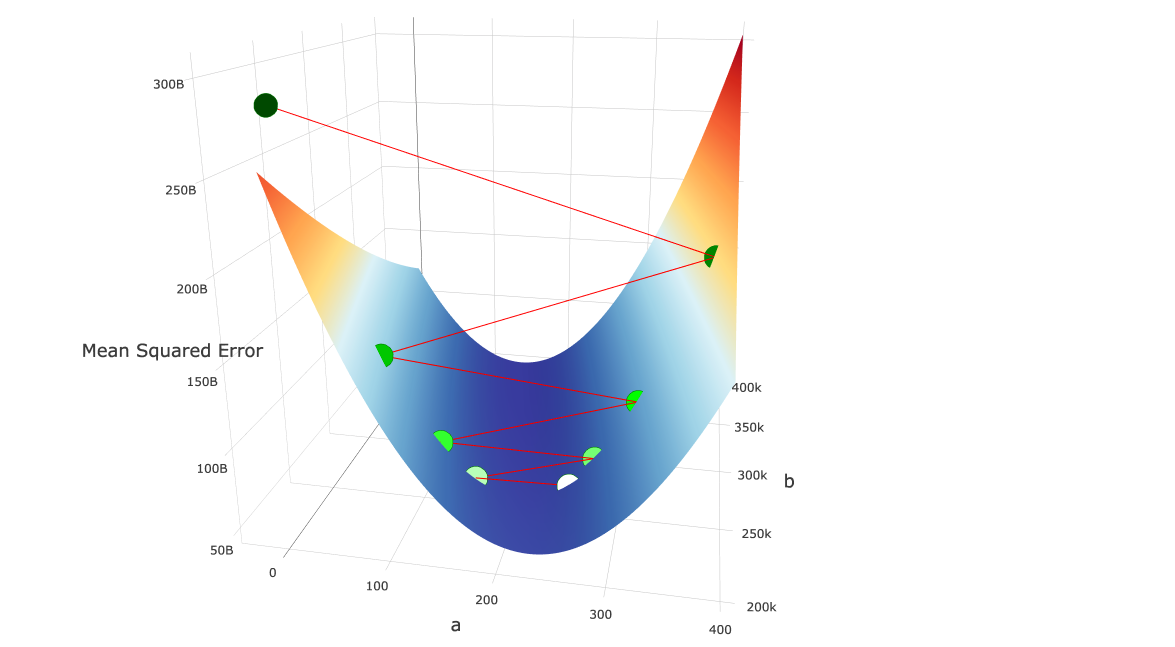
\includegraphics[scale = 0.5]{gradient.png}
\end{figure}
Prácticamente, haces que este rebote hasta que desciende lo suficiente.

\section{Objetivos:}
\subsection{Objetivo general:}
\subsection{Objetivo particulares:}
\begin{itemize}
\item
\end{itemize}
\section{Desarrollo:}
\section{Conclusión:}
\section{Referencias:}
\begin{itemize}
\item Wikipedia contributors. (2022). Mean squared error. Wikipedia.
  \url{https://en.wikipedia.org/wiki/Mean_squared_error}
\item Wikipedia contributors. (2023a). Linear regression. Wikipedia.
  \url{https://en.wikipedia.org/wiki/Linear_regression}
\item Wikipedia contributors. (2023b). Notation for differentiation. Wikipedia.
  \url{https://en.wikipedia.org/wiki/Notation_for_differentiation}
\item Wikipedia contributors. (2023a). Gradient. Wikipedia. \url{https://en.wikipedia.org/wiki/Gradient}
\item Wikipedia contributors. (2023). Loss function. Wikipedia. 
	\url{https://en.wikipedia.org/wiki/Loss_function}
\end{itemize}

\end{document}

